\pagestyle{Uni}

\chapter{Improvements}

Since the application was developed in a very short period of time there are some improvements that could benefit the application. This chapter will list some ideas for these improvements.

\section{Monster drops items}
The team like the idea of items scattered around on the map, but would also like monster to have a chance to drop items when they are killed. Since some items are better than others a looting system in some format would be required.

\section{Monster and item class type}
It is currently possible to spawn three different monster class': 'Common', 'Epic' and 'Boss'. However, the class type is only known at spawn time. As soon as the monster is in the list there is no way to check the class type unless one checks on the name. \\
The same problem is present for items, but here one can't even spawn class type, since it's currently totally random. Therefore it would benefit the gameplay experience to serve the class type info to the player via the fragment (See figure \ref{fig:classTypeCommon} and \ref{fig:classTypeLegendary}). This will also give some better balancing options for the game in case we introduce monster drops etc. so the chance of getting a legendary item is less likely than a simple common sword.

\begin{figure}[ht!]
	\centering
	\begin{minipage}[b]{0.48\textwidth}
		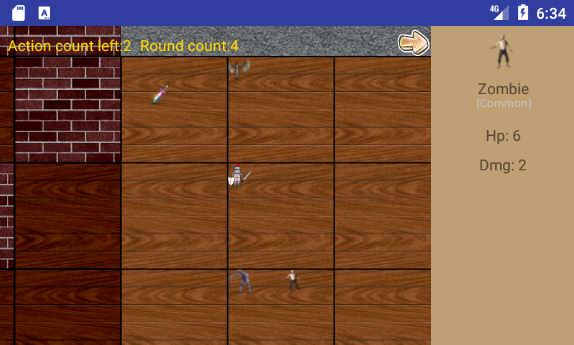
\includegraphics[width=\textwidth]{images/ClassImprovementCommon.png}
		\caption{Common monster}
		\label{fig:classTypeCommon}
	\end{minipage}
	\hfill
	\begin{minipage}[b]{0.48\textwidth}
		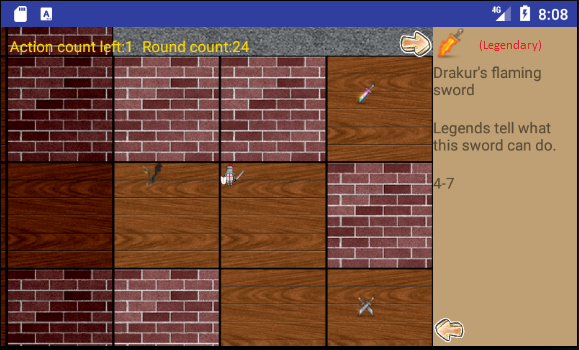
\includegraphics[width=\textwidth]{images/ClassImprovementLegendary.png}
		\caption{Legendary weapons}
		\label{fig:classTypeLegendary}
	\end{minipage}
\end{figure}

\section{Update fragment automatically}
When a player losses health or gain a new item the fragment does not reflect this automatically. Currently, the player has to reopen the fragment in order to get that information. An obvious improvement would therefore to make this happen automatically.\\
This could be done in two ways. Either a similar approach as the item listener, were the activity has the responsibility to update the fragment, or by letting the fragment implement a local broadcast receiver and thereby moving the responsibility into the fragment itself. The last one is the preferred way, since it would make the activity responsible for knowing what to show, but let the fragment be responsible for keeping it up to date.

\section{Different types to items}
The current game only has weapons as items. However, more items will be included in the future. This is also the reason that ItemWeapon class inherit from GameItem class as shown in figure \ref{fig:itemsAndMonstersDiagram}. An example would be armor, that therefore also would inherit from GameItem class.

\section{Firebase synchronisation}
When two or more players take an action at the same time only one would actually take place, the rest would reset their actions. This is both quite annoying for the users but it also introduces some potentially errors since each game state list is maintained asynchronously and separately; One list might get updated correctly, but the others reset. This bug/feature are explained in depth in chapter \ref{ch:knownBugs}. 